% !TeX root = ..\Report.tex
\chapter{Contexte général du projet}

Ce chapitre présente l’organisme d’accueil Orange Business Maroc, ses différentes entités, l’organisation hiérarchique. 
Ensuite, on va présenter le projet de fin d’études, son contexte, ses objectifs et les motivations qui ont poussé à sa réalisation.

\clearpage

\section{Introduction}

L'objectif est de présenter l'organisme d'accueil \textbf{Orange Business Maroc}, son historique, l'organisation hiérarchique, ainsi qu'une description de sa vision stratégique.

\section{Organisme d’accueil}

%\subsection{Presentation de l’organisme}

Orange Business est l’entité du Orange qui est une entreprise française. 
Elle a pour mission de réaliser les mandats de transformations numériques. 
Nous allons commencer par présenter la société mère puis nous allons présenter l’organisme d’accueil.

\subsection{France Télécom}

France Télécom est une société française de télécommunications et la 121e entreprise mondiale. 
Elle emploie près de 172 000 personnes, dont 105 000 en France, et sert près de 226 millions de clients dans le monde. 

\subsection{De France Télécom à Orange}

France Télécom a progressivement laissé place à la marque Orange dans le domaine des télécommunications en France. 
Ce changement majeur a conduit à une transformation significative de la structure et des services offerts par l'entreprise.

\begin{itemize}
    \item À la fin des années 80, avec l'ouverture du marché des télécommunications à la concurrence, France Télécom est créée comme société de service public, principalement détenue par l'État. Elle reprend les activités de télécommunications autrefois gérées par les PTT.
    \item Parallèlement, Orange est fondée au Royaume-Uni en 1994, initialement spécialisée dans la téléphonie mobile.
    \item En 2000, France Télécom acquiert la marque Orange, fusionnant avec elle en 2003.
    \item En 2004, France Télécom devient une entreprise privée, et progressivement tous ses services sont commercialisés sous la marque Orange.
    \item La transition complète vers le nom Orange est effectuée à partir de 2013.
\end{itemize}

\subsection{Le groupe Orange}

Orange est devenu l'un des leaders du marché des télécommunications en France, avec l'un des réseaux les plus performants du territoire. Ses services couvrent la téléphonie fixe et mobile, l'accès à internet, la télévision, la banque en ligne, ainsi que des solutions spécifiques pour les professionnels et les entreprises.
Les services d'Orange s'étendent également à l'international, avec plus de 260 000 clients dans une trentaine de pays en Europe, en Afrique et dans le monde.

En décembre 2019, Orange a présenté son nouveau plan stratégique intitulé \textbf{"Engage 2025"}. Ce plan vise à
réinventer le métier d’opérateur du groupe. 

\noindent Cette nouvelle stratégie vise à accélérer le développement de
nouveaux projets dans les pays à fort potentiel de croissance et à placer la data et l’IA au cœur de son modèle
d’innovation.

\medskip

Le tableau ci-dessus présente une fiche d’identité du groupe Orange.

\begin{table}[h]
\centering
\begin{tabularx}{\textwidth}{|X|X|}
\hline
\textbf{Nom de l’entreprise} & ORANGE \\
\hline
\textbf{Forme juridique} & SA à conseil d’administration \\
\hline
\textbf{Directeur Général} & Christel Heydemann \\
\hline
\textbf{Date de création} & 01-01-1991 \\
\hline
\textbf{Adresse postale} & 111 QUAI DU PRESIDENT ROOSEVELT 92130 ISSY-LES-MOULINEAUX \\
\hline
\textbf{Activité} & Telecom \\
\hline
\textbf{Nombre d’employés} & 136 000 salariés \\
\hline
\textbf{Chiffre d’affaires 2023} & 44 100 000 000.00 \euro{} \\
\hline
\end{tabularx}
\caption{Fiche d’identité groupe Orange}
\label{tab:my_label}
\end{table}

\subsection{Vision du groupe Orange}

Dans sa stratégie de développement et d’évolution, l’ambition du Groupe Orange repose sur cinq leviers d’actions et une dynamique d’un groupe digital efficace et responsable. 
Ces objectifs qui régissent le travail quotidien de tous ces collaborateurs sont comme suit :

\begin{itemize}
    \item Garantir une connectivité enrichie, plus performante sur tous les niveaux et plus
    écologique le tout sans frontières.
    \item Elaborer un modèle d’employeur digital et humain, et offrir une expérience employé
    unique alimentée par le digital et suscitant l’engagement.
    \item Assister la transformation des entreprises clientes, pour suggérer de nouvelles mé-
    thodes de travail et mettre la technologie au service des projets relatifs à la trans-
    formation.
    \item Se diversifier en tirant parti de ses actifs, et des marchés porteurs d’avenir, tels que
    les services bancaires mobiles et les objets connectés.
\end{itemize}

\subsection{Présentation d’Orange Business}

Profitant de l’envergure du \textbf{Groupe Orange}, \textbf{Orange Business} est une entreprise de services digitaux née du réseau le 1er juin 2006, possédant aujourd’hui tous les outils nécessaires pour conquérir le marché \textbf{B2B}. 
Elle est distinguée par la rigueur d’un opérateur de réseaux leader dans le monde et l’agilité d’un intégrateur de solutions numériques, et propose ainsi un large panel de services IT pour ses clients avec des solutions complètes solides et fiables allant du consulting à l’intégration. 

\begin{figure}[h]
    \centering
    
\includegraphics[width=0.5\textwidth]{logos/OBS.png}
    \caption{Logo Orange Business}
    \label{fig:orange_logo}
\end{figure}

\clearpage

Aujourd'hui, Orange Business, en tant qu'entreprise de services numériques natifs du réseau, est présente dans plus de 65 pays et territoires et compte plus de 30 000 collaborateurs. Elle applique des normes élevées de fiabilité et de performance pour accélérer son développement dans les services informatiques.

\medskip

Dans le cadre du plan stratégique du Orange, \textbf{"Engage 2025"}, Orange Business ambitionne de devenir un leader mondial des services de transformation numérique.
Cette transformation a nécessité une politique ambitieuse d'acquisitions dans les domaines du cloud computing, des données et de la cybersécurité. Au fil des années, les activités \textbf{B2B} d'Orange Business sont devenues un moteur de croissance pour le groupe Orange, qui envisage de poursuivre son développement dans les services d'intégration.

\subsection{Orange Business au Maroc}
Nouvellement créé à Rabat, c’est l’un des 8 centres de services d’OBS implantés dans 8 pays répartis sur 4 continents
dans le monde, un choix stratégique pouvant aider à répondre aux évolutions du marché en termes de services
tout en étant très compétitif, en optimisant les couts et en recrutant les compétences là où elles se trouvent.

\medskip

L’année 2023 a été marquée par des chiffres clés illustrant le rôle central d’Orange Business Maroc dans l’écosystème numérique marocain. 
Avec un chiffre d’affaires de 64 millions d’euros, et 980 salariés, dont 45\% de femmes, et un âge moyen de 31 ans, 
l’équipe d’Orange Business Maroc incarne l’excellence et l’innovation, 
prête à relever les défis de la transformation numérique avec agilité et dynamisme.

\medskip

L'extrait ci-dessus présente les entités opérationnelles d'Orange Business Maroc:

\begin{figure}[h]
    \centering
    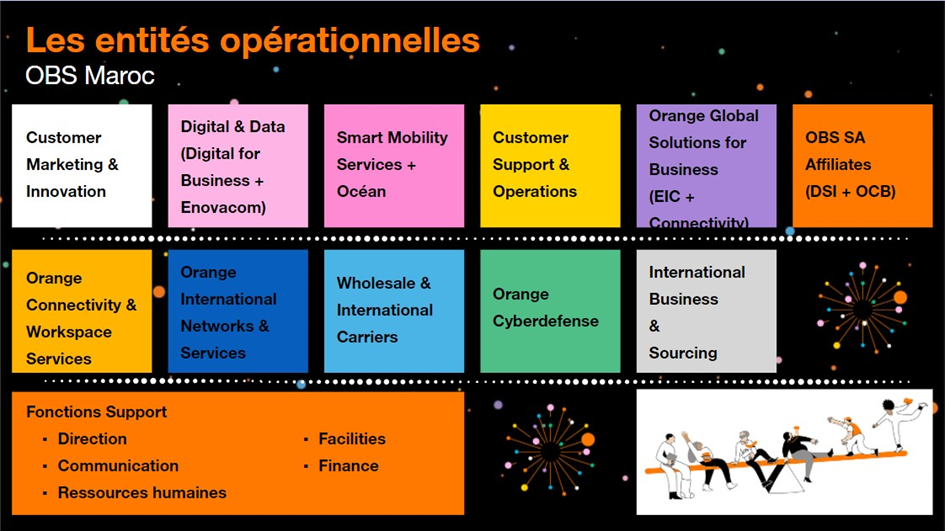
\includegraphics[width=1\textwidth]{images/entités_opérationnelles.png}
    \caption{Les entités opérationnelles d’OB Maroc}
    \label{fig:obs_it_entites}
\end{figure}

\section{Ecosystème Orange Business Maroc}
%\subsection{Organisation et organigramme}
Orange Business MAROC chapeautée par une directrice \textbf{Mme. Rym Sahnoun} qui est l’instance
suprême, est organisée en pôles opérationnels dont le but est de focaliser au quotidien ses
énergies vers la satisfaction de sa clientèle.

\medskip

Ce projet de stage PFE a été effectué au sein de l'entité \textbf{CTIO}, anciennement \textbf{OBS IT}, gérée par \textbf{M. Aarab Abderrahim}. 
Plus précisément, le stage s'est déroulé dans le département \textbf{Customer Marketing Innovation}, au sein de l'équipe \textbf{IMSM Monitoring}. 
Cette équipe fait partie du secteur \textbf{IT OSS} (Operations Support Systems) et est rattachée à \textbf{Mme. ELFAGHLOUMI Asmae}, 
Manager du portefeuille B2B \textbf{Gestion des Incidents, Supervision et Maintenance}, qui fait partie du train safe du \textbf{Monitoring}.

\subsection{Customer Marketing Innovation (CMI)}
Afin de s’adapter aux changements rapides des pratiques de travail internes et de faire face à
la concurrence accrue des nouveaux acteurs numériques, Orange Business doit accélérer sa propre transformation numérique et concentrer ses efforts sur l’amélioration de l’expérience utilisateur.

\medskip

La direction d’Orange Business a créé en 2018 une direction du marketing, de la communication, de l’innovation et du numérique. 
La direction générale d’OB vise à renforcer la place du client au cœur de la transformation numérique. 
Cette entité est appelée Customer Marketing and Innovation (CMI). 
L’entité CMI vise à répondre aux objectifs suivants pour Orange Business :

\begin{itemize}
    \item \textbf{Améliorer l’expérience client} : Avec un accent particulier sur la qualité des services en France et
    avec la consolidation des initiatives existantes pour accélérer la mise en œuvre d’un plan d’amélioration
    commun.
    \item \textbf{Une stratégie marketing plus transversale} : pour développer les domaines stratégiques et agir
    comme un véritable différenciateur en développant un discours commun pour toutes les entités et activités.
    \item \textbf{Une stratégie de communication plus intégrée} : en alignant les programmes de communication
    interne et externe pour refléter la vision d’OBS, encourager le partage des connaissances et développer
    les compétences.
    \item \textbf{Une approche plus visible de l’innovation} : en s’appuyant sur les capacités d’innovation d’OB, du
    groupe Orange, des partenaires et des clients pour créer un différenciateur clé face aux concurrents,
    tout en encourageant et en mettant en valeur l’innovation des employés.
    \item \textbf{Accélérer la transformation numérique d’Orange Business} : tant pour les clients que pour les processus internes, 
    en étant plus centré sur l’utilisateur ; en s’appuyant sur la transformation et sur de nouvelles méthodes agiles de travail.
\end{itemize}

\medskip

Cette entité adopte un modèle de livraison agile, possède un environnement 
de développement et de production simple et automatisé. Il s’agit d’une équipe
polyvalente, autonome et engagée pour gérer l’ensemble des activités relatives aux 
applications qui lui sont confiées : de la collecte des besoins et exigences des clients, à la
rédaction des user stories, en passant par le développement, le test et l’intégration, avant
d’arriver au déploiement et au support.

\clearpage

La figure en bas présente les différentes divisions de la direction CMI.

\begin{figure}[h]
    \centering
    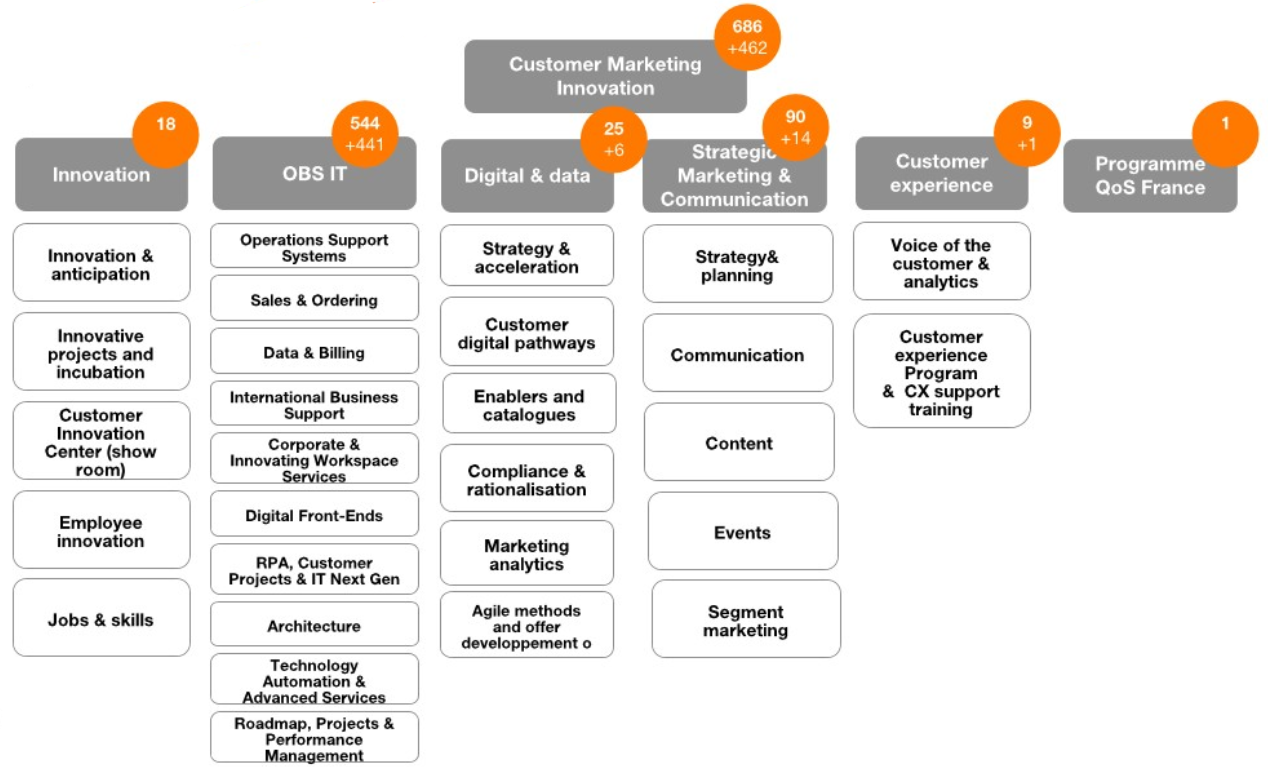
\includegraphics[width=1\textwidth]{images/cmi_entity.png}
    \caption{Organigramme du CMI}
    \label{fig:cmi_organigrame}
\end{figure}

\subsection{CTIO - OBS IT}
CTIO, anciennement OBS IT Morocco est fondé pour reprendre en main ses applications, optimiser et
rationaliser les coûts et rapprocher les équipes de développement des directions métiers et
pour améliorer les délais de livraison des solutions IT pour les TTM(Time to Market). En suivant un mode
de fonctionnement Agile pour livrer de manière régulière les fonctionnalités qui créent le
plus de valeur et en adoptant un Environnement de développement et production simple
et automatisée pour se focaliser sur l’essentiel. 

OBS IT Morocco utilise le cloud, les outils DevSecOps, et tests automatique et l’utilisation des feedbacks pour enrichir 
les applications en veillant à mettre au centre l’expérience utilisateur. En garantissant des équipes
polyvalentes, autonomes et engagées pour gérer toutes les activités sur leur applications
(collecte des besoins rédaction des US, développement, tests intégration, déploiement
support).

Elle représente la direction du système d’information d’Orange Business. Ces missions majeures sont :
\begin{itemize}
    \item Développer, produire et exploiter les applications SI pour les utilisateurs internes et pour les clients externes (portails et interfaces digitales).
    \item Fournir et supporter l’environnement de travail des salariés d’Orange Business.
    \item Définir la politique technique IT : Architecture SI, standard de développement et d’exploitation (Devops, API, Cloud.).
\end{itemize}

\clearpage

L’image ci-après annonce les différentes branches/ secteurs de CTIO (OBS IT).

\begin{figure}[h]
    \centering
    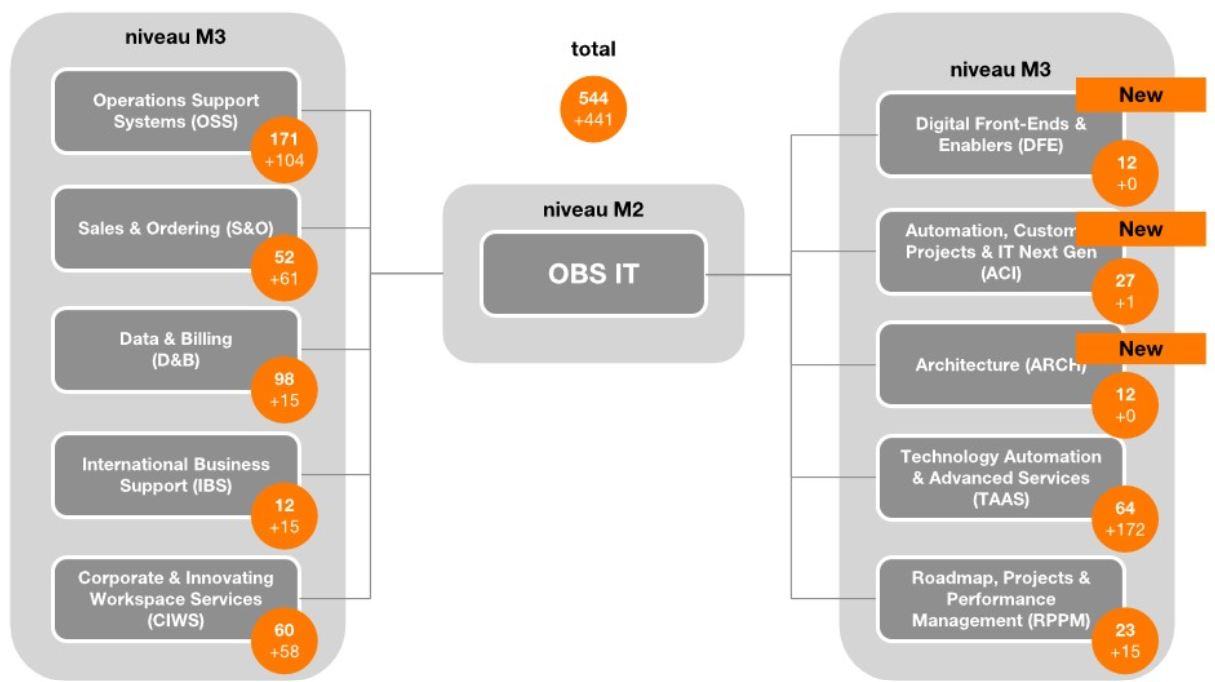
\includegraphics[width=1\textwidth]{images/ctio_direction.png}
    \caption{Organigramme de CTIO}
    \label{fig:ctio_organigrame}
\end{figure}

Les principaux secteurs de CTIO sont :

\begin{itemize}
    \item \textbf{Operation Support Systems (OSS)}: Sa mission c’est l’IT, de la prestation de services au suivi et au soutien.
    \item \textbf{Data \& Billing (D\&A)}: Ses mission c’est d’améliorer la gestion des données et participer à la révolution des données/IA via une plateforme permettant la création de valeur pour les clients d’OBS et pour les employés. Aussi d’améliorer l’expérience et la confiance des clients grâce à des données fiables fournies par les meilleurs services de facturation opérationnels, sécurisés et prêts pour le numérique.
    \item \textbf{International Business Support (IBS)}: Gérer les outils de cotation pour soutenir les BU et les canaux d’OBS Marketing dans leur activité commerciale.
    \item \textbf{Corporate \& Innovative Workspace Services (CIWS)}: Moderniser et transformer l’espace de travail des employés, développer des solutions innovantes pour la communication. Gérer le service IT des parties prenantes de l’entreprise (RH, Finance et juridique).
    \item \textbf{Digital Front-End \& Enablers(DFE)}: Simplifier et proposer des parcours clients de premier ordre pour les principaux parcours numériques. Améliorer la satisfaction des clients et des employés. Soutenir l’ambition des projets clients d’OBS IT.
    \item \textbf{Automation,Customer Projects \& IT Next Gen (ACI)}: Intégrer de manière transparente l’ensemble des technologies disponibles et en y ajoutant une couche d’intelligence pour une meilleure expérience du consommateur.
    \item \textbf{Architecture (ARCH)}: Apporter un soutien sur l’architecture fonctionnelle transversale.
    \item \textbf{Technology Automation \& Advanced Services (TAAS)}: Fournir les meilleurs outils techniques et le meilleur soutien pour faciliter la transformation technologique en garantissant la qualité de service et la sécurité des échanges inter-entreprises (E2E).
    \item \textbf{Roadmap ,Projects \& Performance Management (RPPM)}: L’objectif est d’aligner la feuille de route sur les plans stratégiques des parties prenantes, de soutenir toutes les initiatives de transformation technologique et humaine de l’entreprise, et de piloter le budget et les performances par le biais d’une gouvernance de projet commune.
\end{itemize}

\subsection{Portefeuilles B2B de CTIO Maroc}

L'Agilité BtoB est une approche qui vise à appliquer les principes et pratiques agiles dans un contexte Business-to-Business. 
Cette approche se concentre sur la livraison rapide de valeur aux clients, l'adaptabilité et la collaboration inter-entreprises.

\medskip

La mise en œuvre des chaînes de valeur en portefeuilles pour le B2B a donné lieu à la création de ces 12 portefeuilles fonctionnels.

\begin{figure}[h]
    \centering
    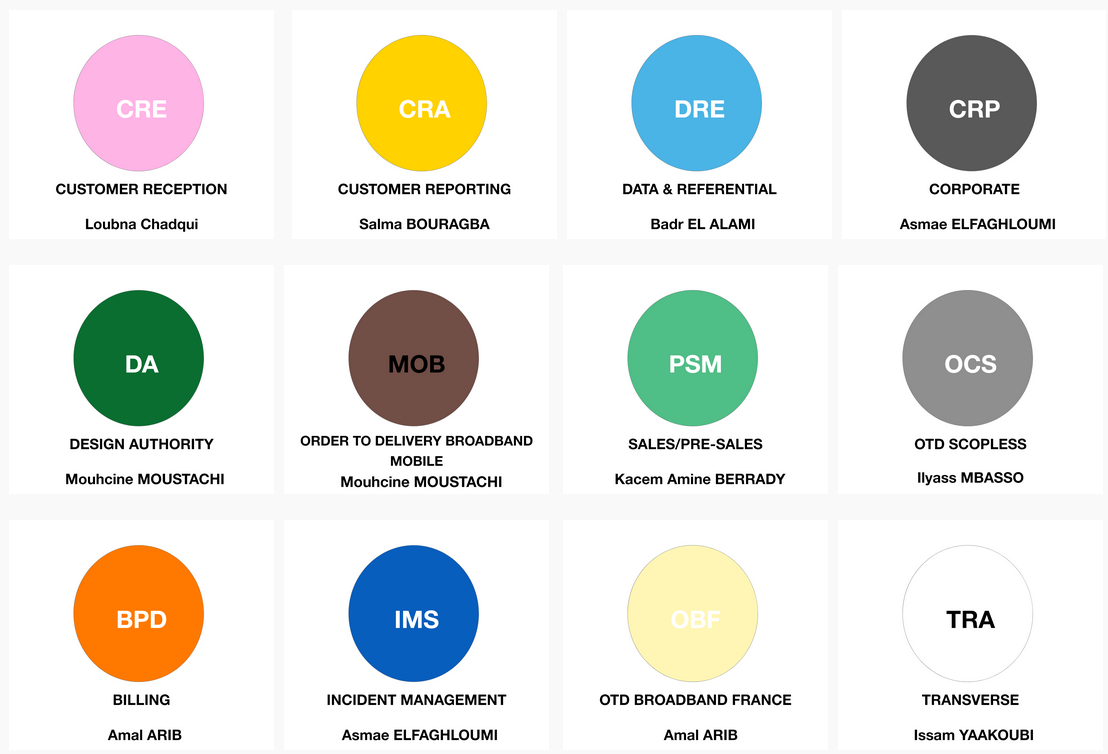
\includegraphics[width=1\textwidth]{images/ctio_portefeuilles.png}
    \caption{Les portefeuilles occupés par CTIO Maroc}
    \label{fig:ctio_portefeuilles}
\end{figure}

\medskip

Orange Business CTIO Maroc prend en charge ces portefeuilles sous sa tutelle.
Mon stage PFE s’est déroulé au niveau d’un projet de monitoring '\textbf{Watch}' du portefeuille "\textbf{Gestion des Incidents, Supervision et Maintenance}".

\subsection{Train Safe de Monitoring}
Un train (Agile Release Train dans SAFe) est un dispositif permettant la coordination, le cadencement et l’alignement de plusieurs équipes agiles pour la réalisation d’une solution commune. 

\begin{figure}[h]
    \centering
    
\includegraphics[width=0.8\textwidth]{images/train_BtoB.png}
    \caption{Train Business to Business}
    \label{fig:train_b2b}
\end{figure}

Il intègre également des rôles dédiés à son fonctionnement :

\begin{itemize}
    \item \textbf{Release Train engineer (RTE)}: Il est au service des équipes du train agile et il y incarne les valeurs de l'agilité. Il est le facilitateur du train.
    \item \textbf{Product Management (PM)}: Il porte la vision des évolutions de la solution et s'assure qu'elle apporte le maximum de valeur pour les clients/utilisateurs et le business. Il représente le client, comprend ses besoins et valide les solutions proposées.
    \item \textbf{System Architect (SA)}: Il définit les orientations architecturales, techniques et d'infrastructure de la solution répondant à la vision business du train.
    \item \textbf{Business Owner (BO)}: Ils sont un petit groupe de parties prenantes qui ont la responsabilité de maximiser le ROI de la solution développée par un Agile Release Train (ART) tout en s'assurant de la conformité de la solution. Ils sont des parties prenantes clés de l'ART qui doivent évaluer l'aptitude à l'usage de la solution et participer activement à certains événements.
\end{itemize}

Train Safe de Monitoring regroupe des équipes qui travaillent ensemble pour concevoir, développer, intégrer et opérer une solution de monitoring des produits IT, Network ou Sécurité d'Orange Business. 

\noindent L'objectif principal de ce train est de répondre aux attentes et aux standards du marché en fournissant une solution de monitoring de haute qualité pour les clients externes et les équipes opérationnelles internes.

\medskip

Les équipes '\textbf{IMSM-Monitoring}' sont également intégrées dans le train Safe de Monitoring, afin de garantir une coordination et une collaboration efficaces entre les différentes équipes travaillant sur les projets de monitoring.
Les équipes projet concernées incluent \textbf{MUSE}, \textbf{WATCH}, \textbf{TCS}, \textbf{Self Monitoring}, \textbf{AIOps}.

\clearpage

\subsection{Équipe WATCH}

\begin{figure}[h]
    \centering
    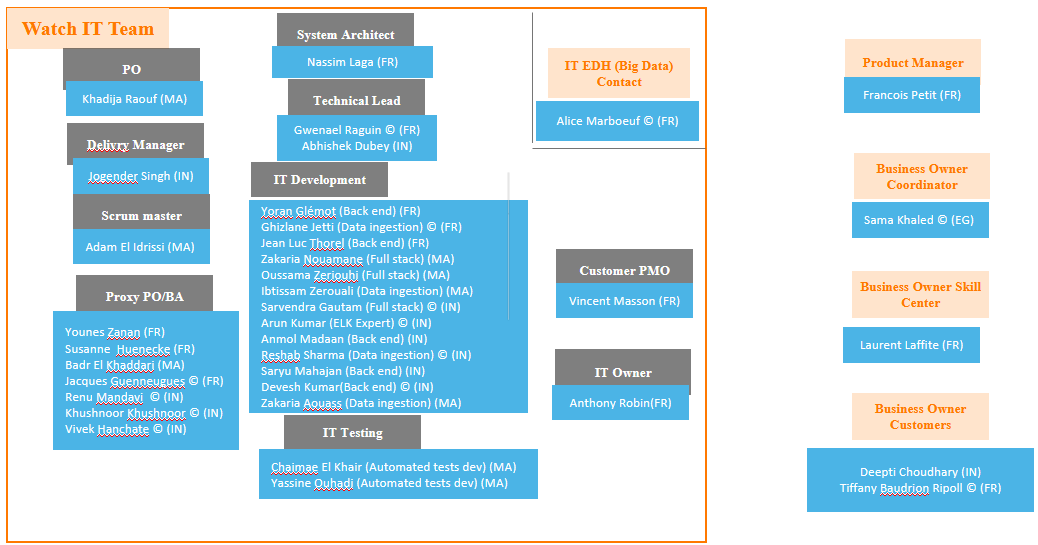
\includegraphics[width=1\textwidth]{images/watch_team.png}
    \caption{L'Équipe WATCH}
    \label{fig:watch_team}
\end{figure}

\section{Conclusion}